% !TEX root = Skin_Lesion_Classification_Using_Machine_Learning.tex

\section{Introduction [TN, SE]}\label{sec:introduction}
%#TODO: Motivation for Machine Learning, describing the unknown class problem
Skin cancer is one of the most common types of cancer. It makes up more then half of the worldwide cancer diagnoses. Melanoma is the most dangerous type of skin cancer that can arise through different causes. A mole can change over time with an increase in size, irregular edges, change in color, itchiness or skin breakdown \cite{Zaqout19}. The primary cause of melanoma is the influence of ultraviolet light exposure from the sun or other sources like tanning devices. Its incidence and mortality rates have been increasing in the last decades \cite{Lens04} and therefore it represents an important public health problem. In 2012 out of 232,000 people that were diagnosed with Melanoma 55,000 people died. \\
However, if skin cancer is diagnosed in an early stage, it has very high curing rates. To detect cancerous skin dermatologists usually evaluate a skin lesion with the so called ABCD rule \cite{Stolz94}. In the first step the "\textbf{a}symmetry, \textbf{b}order, \textbf{c}olors, and \textbf{d}iameter" criteria are approximately estimated. In the second step each criteria is multiplied by a given weight factor to get the total dermoscopy score. This shows the importance of the shape and texture of the lesion in skin cancer diagnoses.\newline \newline
In this work we will use machine learning techniques to classify the type of skin lesion based on skin lesion images. For the required data we use the ``ISIC 2019: Training'' dataset that was published by the International Skin Imaging Collaboration (ISIC). This dataset contains 25,331 images of 8 different types of skin lesions. The test dataset also contains additional skin images that don't fall in any of there categories. Those images are referred to as unknown. 
The dataset is composed of three separate sources. Part of the data originates from the HAM1000 dataset \cite{HAM10000}. Those images are of size $600 \times 450$ and were manually cropped around the lesion by the dataset creators. Some of the images are also preprocessed by histogram equalization. % #TODO where to put the citation? This is all based on \cite{HAM10000}
The second dataset is the BCN20000 dataset \cite{bcn20000} containing high resolution images ($1024 \times 1024$). Not all images of that dataset are cropped, meaning there are images present with large black borders and the skin only visible in a circle in the middle. The last dataset is the MSK dataset \cite{MSK_Data} with images of different sizes originating from several sources. 
Table \ref{tab:data} shows the name of the lessions together with the number of images of these classes in the training dataset.

\begin{table}[ht]
    \caption{Number of samples per class in the training dataset}
    \begin{center}
    \begin{tabular}{c|c}
        \hline
        \textbf{Lesion}&\textbf{Number of samples} \\
        % \hline
        0-Melanoma &  4522 \\
        % \hline
        1-Melanocytic nevus & 12875  \\
        % \hline
        2-Basal cell carcinoma & 3323 \\
        % \hline
        3-Actinic keratosis & 867 \\
        % \hline
        4-Benign keratosis & 2624 \\
        % \hline
        5-Dermatofibroma & 239 \\
        % \hline
        6-Vascular lesion & 253 \\
        % \hline
        7-Squamous cell carcinoma & 628 \\
        % \hline
        8-Unknows & 0 \\
        \hline
    \end{tabular}
    \label{tab:data}
    \end{center}
\end{table}

As seen in the table, the dataset is heavily imbalanced. To get meaningful evaluation results, we rate our approaches using the  balanced multi-class accuracy, wich is equivalent to the macro-average sensitivity, as our main metric \cite{Mosley2013}. 
% #TODO maybe move to a better location?

Four images and the belonging classes are illustrated in figure \ref{fig:dataset}.
% #TODO select more meaningful images (with hair, cropped/not cropped, ...)
\begin{figure}
	\begin{subfigure}{.24\textwidth}
		\centering
		% include first image
		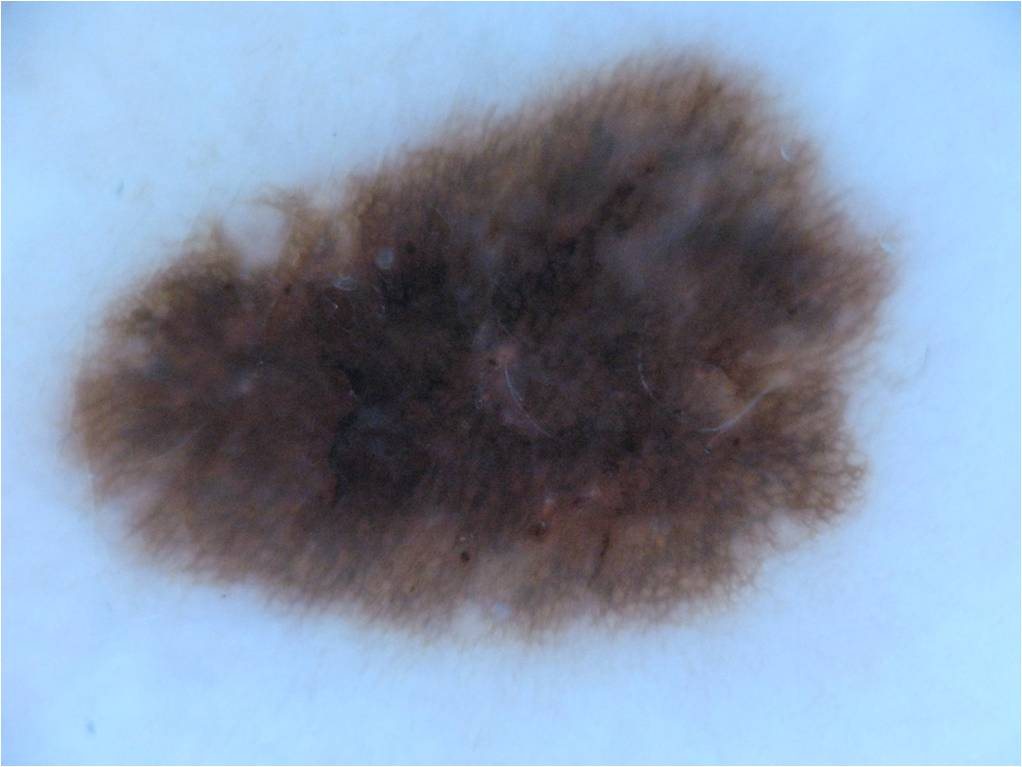
\includegraphics[width=.9\linewidth]{pictures/ISIC_0000000.jpg}  
		\caption{ISIC\_0000000: class 1}
		\label{fig:sub-first}
	\end{subfigure}
	\begin{subfigure}{.24\textwidth}
		\centering
		% include second image
		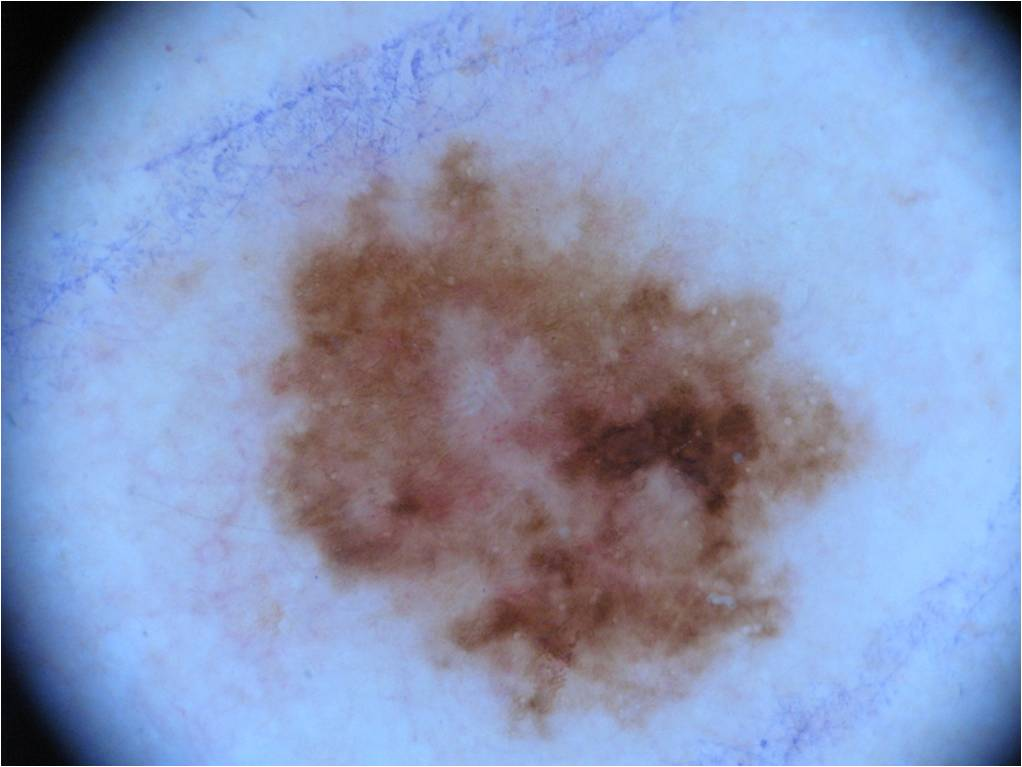
\includegraphics[width=.9\linewidth]{pictures/ISIC_0000002.jpg}  
		\caption{ISIC\_0000002: class 0}
		\label{fig:sub-second}
	\end{subfigure}
	
	\begin{subfigure}{.24\textwidth}
		\centering
		% include third image
		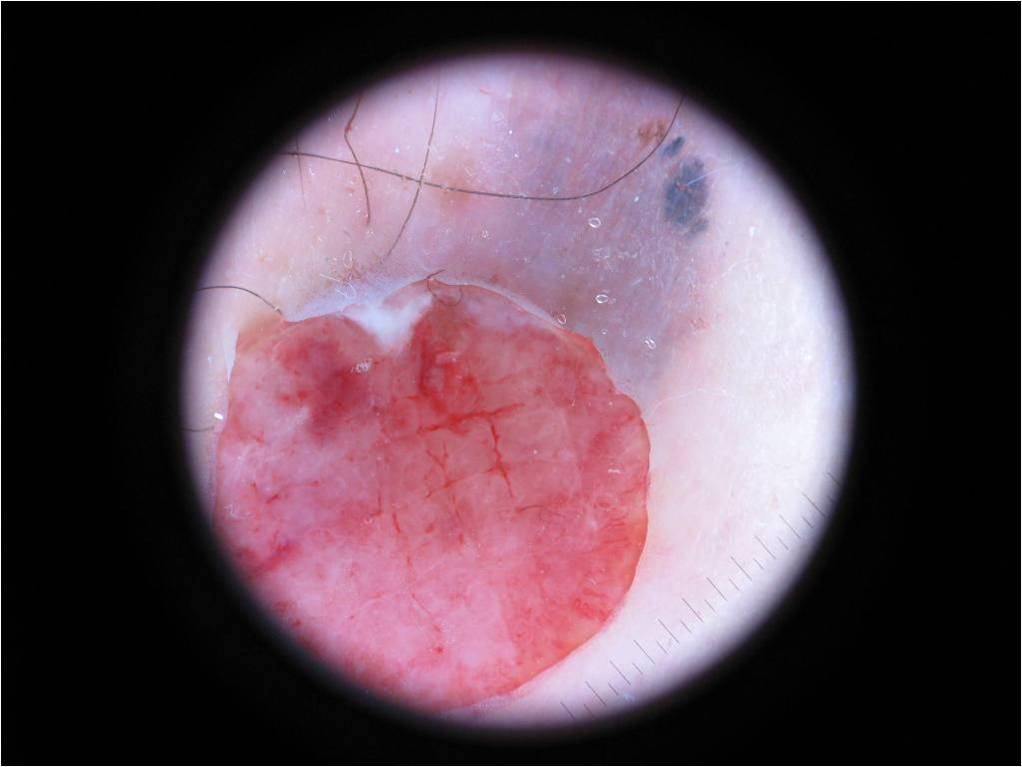
\includegraphics[width=.9\linewidth]{pictures/ISIC_0000004.jpg}  
		\caption{ISIC\_0000004: class 0}
		\label{fig:sub-third}
	\end{subfigure}
	\begin{subfigure}{.24\textwidth}
		\centering
		% include fourth image
		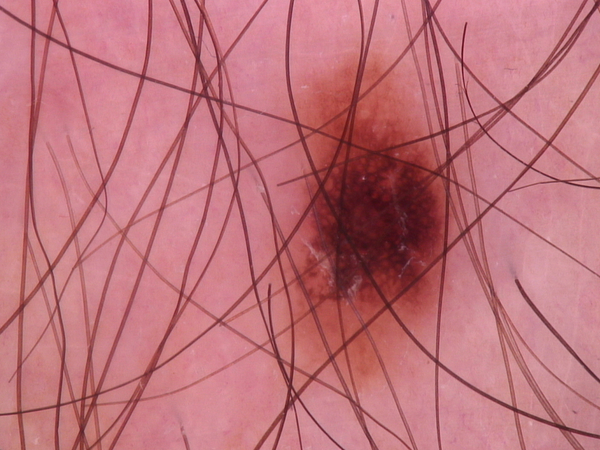
\includegraphics[width=.9\linewidth]{pictures/ISIC_0026767.jpg}  
		\caption{ISIC\_0026767: class 1}
		\label{fig:sub-fourth}
	\end{subfigure}
	\caption{Four images of the ``ISIC 2019: Training'' dataset.}
	\label{fig:dataset}
\end{figure}
%Only the skin lesion itself is interesting for the classification, not the normal skin around it or hair that covers the lesion.\\
There is also additional data for most images called meta data. This contains information of the age and gender of the belonging patient and the position of the skin lesion on the patients body. 
For the skin lesion classification we will present two different approaches: \\
In section \ref{sec:svm} we are using Support Vector Machine (SVM) for the classification. Therefor data preprocessing and feature extraction is necessary. These features describe the shape and texture of the image and are used as input data.
% This procedure can be seen in figure \ref{fig:intro_svm}.\\
In the following section \ref{sec:cnn} we are using a Convolutional Neural Network (CNN) for the classification. CNNs have become increasingly important in the domain of medical image analysis. Here the image itself is used as the input data. 
% This procedure can be seen in figure \ref{fig:intro_cnn}.
% \begin{figure}[ht!]
% 	%\centering
% 	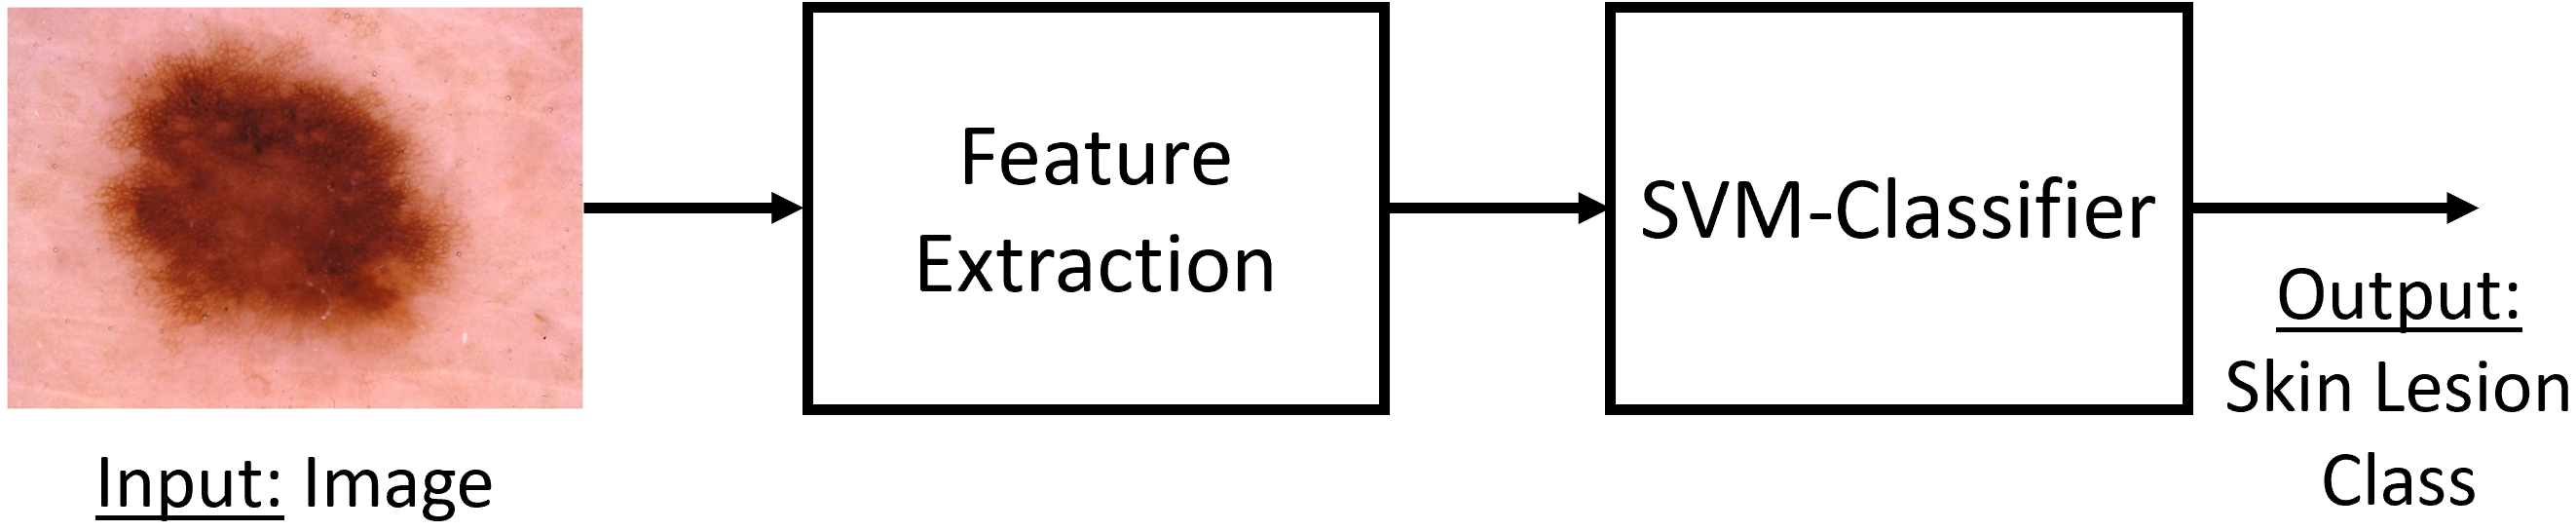
\includegraphics[height=1.8cm]{pictures/intro_01.png} 
% 	\caption{Classification with Support Vector Machine}
% 	\label{fig:intro_svm}
% \end{figure}
% \begin{figure}[ht!]
% 	%\centering
% 	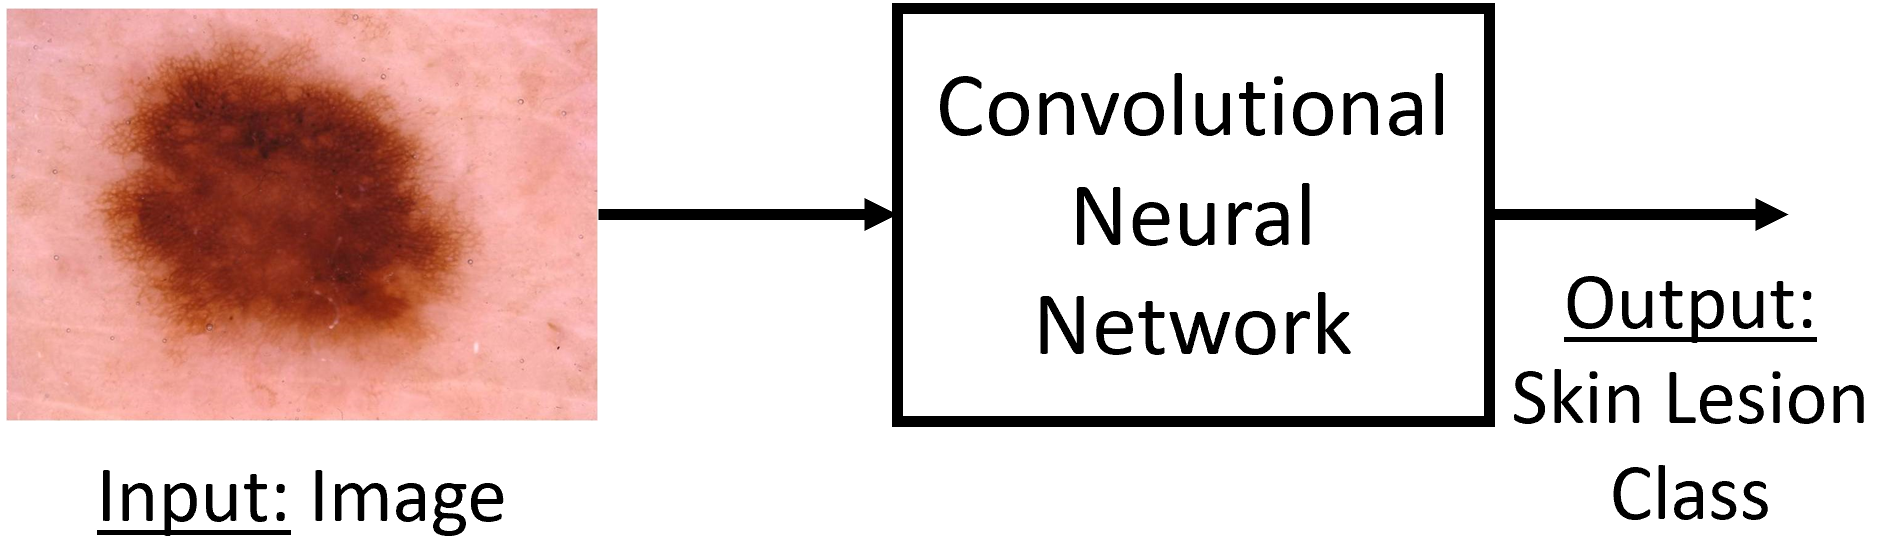
\includegraphics[height=1.8cm]{pictures/intro_02.png} 
% 	\caption{Classification with Convolutional Neural Networks}
% 	\label{fig:intro_cnn}
% \end{figure}
Furthermore we will investigate the prediction results by taking the additional meta data into account. 
One of the main challenges is the classification of the unknown class in the test dataset. Our approach for that is shown in section \ref{sec:unknown_data}.
In the last section \ref{sec:conclusion} we will discuss the two different approaches and summarize our results.
